% Version CoNaIISI 2026 del trabajo sobre Activaciones Racionales
% Condicionadas por Contexto. Basada en el formato oficial del congreso
% (CONAIISI2026_Template), con los paquetes de tablas agregados en format.tex.
%
% Compilar:  pdflatex main && bibtex main && pdflatex main && pdflatex main

\documentclass[10pt,a4paper,final,oneside,notitlepage]{article}
\usepackage[utf8]{inputenc} % Acentos, etc.
\usepackage[T1]{fontenc}    % Silabeo correcto de palabras acentuadas
\usepackage[spanish,es-tabla]{babel} % Idioma español con "Tabla" por defecto

% Márgenes según pautas CoNaIISI:
% Área de impresión: 17,5 cm de ancho por 22,54 cm de alto.
% Columnas de 8,25 cm con 8 mm de separación (8,25 * 2 + 0,8 = 17,3 cm).
% Margen superior e inferior de 3,0 cm en todas las páginas.
% Márgenes laterales: 1,85 cm en cada lado (21,0 cm - 1,85 * 2 = 17,3 cm).
\usepackage[a4paper, left=1.85cm, right=1.85cm, top=3.0cm, bottom=3.0cm]{geometry}
\setlength{\columnsep}{8mm}

% Tipografías según CoNaIISI:
% Texto principal y matemáticas: Times
\usepackage{mathptmx}
% Epígrafes de figuras y tablas: Helvética (Sans-Serif) 9 pts negrita
\usepackage[scaled=0.92]{helvet}
% Código fuente: Courier
\usepackage{courier}

% Paquetes matemáticos y utilidades
\usepackage{amsmath}
\usepackage{amsfonts}
\usepackage{amssymb}
\usepackage{titlesec}
\usepackage{multicol}
\usepackage{cite}        % Citas compactas [1-3], [2, 5]
\usepackage{booktabs}    % Tablas profesionales
\usepackage{multirow}    % Celdas multifila
\usepackage{array}       % Columnas de ancho fijo
\usepackage{setspace}
\usepackage{enumitem}
\usepackage{xcolor}
\usepackage{graphicx}
\usepackage{tikz}

\usepackage[hidelinks]{hyperref} % Hipervínculos en color negro

% Formato de párrafos según CoNaIISI:
% Sangría de 5 mm, completamente justificado, sin espacio adicional entre párrafos.
\setlength{\parindent}{5mm}
\setlength{\parskip}{0pt}

% Epígrafes (Captions) según CoNaIISI:
% Helvética 9 pts negrita.
% Mayúscula solo inicial: "Figura 1. ..." y "Tabla 1. ..."
% Tabla: título centrado por sobre la misma.
% Figura: referencias por debajo de la misma.
\usepackage{caption}
\DeclareCaptionFont{helv9pt}{\fontsize{9pt}{11pt}\selectfont\sffamily\bfseries}
\captionsetup{
  font=helv9pt,
  labelfont=helv9pt,
  labelsep=period
}
\captionsetup[table]{
  position=above,
  skip=6pt,
  justification=centering
}
\captionsetup[figure]{
  position=below,
  skip=6pt,
  justification=centering
}

% Formato de títulos de secciones según CoNaIISI:
% Primer Nivel: Times 12 pts negrita, inicial mayúscula, numerado ("1. Introducción"), ant. 24 pts, post. 12 pts.
\titleformat{\section}
  {\fontsize{12pt}{14.4pt}\selectfont\bfseries}
  {\thesection.\ }
  {0pt}
  {}
\titleformat{name=\section,numberless}
  {\fontsize{12pt}{14.4pt}\selectfont\bfseries}
  {}
  {0pt}
  {}
\titlespacing*{\section}{0pt}{24pt}{12pt}

% Segundo Nivel: Times 11 pts negrita, alineado izquierda, sin sangría, ant. 6 pts, post. 6 pts.
\titleformat{\subsection}
  {\fontsize{11pt}{13.2pt}\selectfont\bfseries}
  {\thesubsection.\ }
  {0pt}
  {}
\titleformat{name=\subsection,numberless}
  {\fontsize{11pt}{13.2pt}\selectfont\bfseries}
  {}
  {0pt}
  {}
\titlespacing*{\subsection}{0pt}{6pt}{6pt}

% Tercer Nivel: Times 10 pts negrita, alineado izquierda, ant. 12 pts, post. 6 pts.
\titleformat{\subsubsection}
  {\fontsize{10pt}{12pt}\selectfont\bfseries}
  {\thesubsubsection.\ }
  {0pt}
  {}
\titleformat{name=\subsubsection,numberless}
  {\fontsize{10pt}{12pt}\selectfont\bfseries}
  {}
  {0pt}
  {}
\titlespacing*{\subsubsection}{0pt}{12pt}{6pt}

% Parámetros de flotantes
\renewcommand{\topfraction}{0.92}
\renewcommand{\bottomfraction}{0.6}
\renewcommand{\textfraction}{0.08}
\renewcommand{\floatpagefraction}{0.7}
\setcounter{topnumber}{3}
\setcounter{totalnumber}{4}

\pagestyle{empty} % Sin número de página

% Notas al pie: Times 9 pts, espaciado simple
\renewcommand{\footnotesize}{\fontsize{9pt}{11pt}\selectfont}

\makeatletter

% Control de versión anónima para revisión por pares (doble ciego):
% \anonimafalse  -> Modo evaluación ciega (oculta autores, filiaciones y repo identificable)
% \anonimafalse -> Modo versión final aceptada (con autores, filiaciones y contactos)
\newif\ifanonima
\anonimafalse

% Metadatos
\def\email#1{\gdef\@email{#1}}
\def\@email{}

\def\universidad#1{\gdef\@universidad{#1}}
\def\@universidad{}

% Título Principal y Autores según CoNaIISI:
% En la primera página debe empezar en el centímetro 3,49 desde el borde superior de la hoja.
% Centrado, Times 14 pts negrita. Mayúscula la primera letra de sustantivos, verbos, etc.
% Dejar dos líneas en blanco (~24 pt) después del título.
% Autores: Times 12 pts estilo normal (sin negrita). Filiaciones: 12 pts cursiva. Email incluido.
% Dejar dos líneas en blanco (~24 pt) antes del texto principal.
\newcommand{\titulo} {
  \begingroup
  \centering
  \vspace*{0.49cm} % 3.0 cm margen superior + 0.49 cm = 3.49 cm al borde superior
  {\fontsize{14pt}{17pt}\selectfont\bfseries\@title\par}
  
  \vspace{24pt}
  
  \ifanonima
    {\fontsize{12pt}{14.4pt}\selectfont\textit{[Artículo remitido para evaluación por pares externos y doble ciego]}\par}
    \vspace{6pt}
    {\fontsize{10pt}{12pt}\selectfont\textit{(Información de autores y filiación omitida según las pautas de evaluación CoNaIISI)}\par}
  \else
    {\fontsize{12pt}{14.4pt}\selectfont\normalfont\@author\par}
    \ifx\@universidad\@empty\else
      \vspace{4pt}
      {\fontsize{12pt}{14.4pt}\selectfont\itshape\@universidad\par}
    \fi
    \ifx\@email\@empty\else
      \vspace{4pt}
      {\fontsize{12pt}{14.4pt}\selectfont\normalfont\@email\par}
    \fi
  \fi
  
  \vspace{24pt}
  \endgroup
}
\makeatother

% Resumen según CoNaIISI:
% Ubicado en la parte superior de la columna izquierda.
% Título "Resumen" con Times 12 pts negrita, centrado en la columna.
% Texto con Times 10 pts cursiva, interlínea simple, justificado.
% Dejar dos líneas en blanco después del resumen (~20 pt).
\newcommand{\resumen}[1]{%
  \begin{center}%
    {\fontsize{12pt}{14.4pt}\selectfont\bfseries Resumen\par}%
  \end{center}%
  \vspace{4pt}%
  {\fontsize{10pt}{12pt}\selectfont\itshape #1\par}%
  \vspace{12pt}%
}

% Palabras clave
\newcommand{\palabrasclave}[1]{%
  \noindent{\fontsize{10pt}{12pt}\selectfont\textbf{Palabras clave---}#1\par}%
  \vspace{16pt}%
}

\newcommand{\miniseccion}[1]{%
  \vspace{6pt}%
  {\fontsize{10pt}{12pt}\selectfont\textbf{#1}\par}%
  \vspace{3pt}%
}

% Entorno de figuras en multicols si se requiere
\newenvironment{Figure}
  {\par\medskip\noindent\minipage{\linewidth}}
  {\endminipage\par\medskip}

% Bibliografía según CoNaIISI: Times 9 pts, espaciado simple, citas entre corchetes
\newcommand{\bibliofont}{\fontsize{9pt}{11pt}\selectfont}

\let\OLDthebibliography\thebibliography
\renewcommand\thebibliography[1]{
  \OLDthebibliography{#1}
  \bibliofont
  \setlength{\parskip}{0pt}
  \setlength{\itemsep}{1pt plus 0.5pt}
}

\title{Activaciones Racionales Condicionadas por Contexto: ¿Cuándo Conviene Adaptar la No Linealidad de una Red?}
\author{Agustín H. Astie Forconesi \quad Juan P. Gerino \quad Joaquín I. Ortega \quad Miguel Méndez Garabetti}
\universidad{Laboratorio de Investigación en Ciencia y Tecnología,\\ Universidad del Aconcagua, Mendoza, Argentina.}
\email{agustinastie3@gmail.com,juanpigerino@gmail.com,joaquinimanolortega@gmail.com,mmendez@uda.edu.ar}

\begin{document}
\titulo

\begin{multicols}{2}

\resumen{
Las redes neuronales profundas aplican la misma función de activación a todas sus entradas, sin importar de qué tipo de datos provengan. Cuando un único modelo debe atender regímenes heterogéneos —imágenes de distintas fuentes, texto de varios dominios, señales capturadas en condiciones diferentes— esa transformación única puede volverse un cuello de botella. Este trabajo investiga si conviene generar la forma de la no linealidad a partir del contexto de cada muestra, y a qué costo. Se propone la Activación Racional Condicionada por Contexto (CCA): una red auxiliar pequeña produce, para cada ejemplo, los coeficientes de una curva racional estable que en la inicialización coincide de manera exacta con la activación SiLU, de modo que el modelo nunca parte de una situación peor que la de referencia. La propuesta se compara con cinco alternativas, entre ellas Dynamic ReLU-B y Meta-ACON, igualando parámetros y operaciones, sobre diez semillas emparejadas y con pruebas exactas corregidas por comparaciones múltiples. En un banco real formado por MNIST, SVHN y USPS, sin informar nunca al modelo de qué conjunto proviene cada imagen, CCA alcanza $88.68\%$ de exactitud y supera a la mejor alternativa por $0.62$ puntos porcentuales. Una matriz de doce tareas adicionales muestra dónde ocurre eso: la ventaja se concentra en las que exigen transformaciones distintas por régimen y se desvanece en las homogéneas. El sobrecosto no es aritmético sino de lanzamiento de núcleos, y la compilación recupera la mayor parte. El resultado es una regla de uso concreta antes que una mejora universal.
}

\palabrasclave{Aprendizaje profundo, Funciones de activación adaptativas, Cómputo condicionado, Hiperredes, Evaluación con presupuesto igualado, Cambio de dominio.}

\section{Introducción}

El aprendizaje profundo debe buena parte de su éxito a unos pocos componentes simples repetidos millones de veces. Entre ellos, la función de activación —la no linealidad que se aplica elemento por elemento entre dos capas— es el más elemental: sin ella, una red de muchas capas colapsa en una única transformación lineal. Desde la adopción masiva de la unidad rectificadora \cite{nair2010relu}, la práctica dominante consiste en elegir una curva fija —ReLU, GELU \cite{hendrycks2016gelu} o SiLU \cite{silu}— y aplicarla de forma idéntica a todas las muestras, capas y situaciones. Esa uniformidad es cómoda, barata y, para datos homogéneos, suficiente.

Los sistemas que se despliegan fuera del laboratorio, en cambio, rara vez observan un único tipo de datos. Un lector de importes recibe cifras manuscritas de un formulario y también fotografías de carteles tomadas con un teléfono; un modelo acústico procesa grabaciones limpias y otras saturadas de ruido. Cada una de esas condiciones —a las que llamaremos \textit{regímenes}— puede requerir una transformación diferente de las mismas características internas, y una activación fija obliga a resolverlas todas con una única curva, es decir, con un compromiso. El problema, además, no se reduce a reconocer el régimen: aun identificándolo, la red necesita \textit{modificar el cómputo} que aplica en consecuencia.

La literatura ofrece dos respuestas parciales. La primera es aprender la forma de la activación durante el entrenamiento, como hacen PReLU \cite{he2015prelu}, Maxout \cite{goodfellow2013maxout}, Swish \cite{ramachandran2017swish}, las unidades racionales \cite{boulle2020rational,molina2020pade} o las redes de Kolmogórov--Arnold \cite{liu2024kan}; en todos esos casos la curva se aprende una sola vez y queda congelada en inferencia, de modo que sigue siendo la misma para todos los regímenes. La segunda proviene del cómputo condicionado \cite{bengio2013conditional}, donde una parte de la red genera o selecciona parámetros de otra: hiperredes \cite{ha2017hypernetworks}, modulación FiLM \cite{perez2018film}, núcleos convolucionales dependientes de la muestra \cite{yang2019condconv} o mezclas de expertos \cite{shazeer2017moe}. En la intersección se ubican Dynamic ReLU \cite{chen2020dynamic} y Meta-ACON \cite{ma2021activate}, que condicionan la activación misma al contenido de la entrada.

Ese cruce deja un vacío que motiva este trabajo. Las ventajas publicadas se miden casi siempre sobre grandes arquitecturas de visión, entre métodos que no comparten presupuesto de parámetros ni de operaciones, y casi nunca vienen acompañadas de controles negativos que muestren dónde la técnica \textit{no} sirve. Uno termina sabiendo que el método ganó, pero no por qué ni a cambio de qué. Falta una respuesta empírica a una pregunta práctica: \emph{¿bajo qué condiciones una no linealidad condicionada por el contexto supera a una fija y a las alternativas dinámicas, cuando todas disponen del mismo presupuesto y el régimen debe inferirse de los datos, sin metadatos que lo revelen?}

Para responderla proponemos la \textit{Activación Racional Condicionada por Contexto} (CCA, por sus siglas en inglés), en la que una red auxiliar diminuta genera, para cada muestra, los coeficientes de una curva racional estable. La utilidad esperada es concreta: mejorar la exactitud de un modelo desplegado sobre datos heterogéneos sin agrandarlo, sin etiquetas de dominio y sin entrenar un modelo por régimen. El aporte se evalúa con dos niveles de evidencia separados: una comparación confirmatoria con presupuesto igualado sobre semillas jamás usadas durante el diseño, y una matriz de doce tareas de visión, lenguaje, audio, razonamiento y generación que incluye controles diseñados para que la técnica pueda fallar.

Las contribuciones del trabajo son cuatro:

\begin{itemize}[leftmargin=1.1em,itemsep=0.15em,topsep=0.25em]
\item una activación condicionada por contexto que se inicializa \textit{exactamente} como SiLU y no puede, por lo tanto, partir en desventaja;
\item una comparación contra Dynamic ReLU-B, Meta-ACON y una racional estática con parámetros y operaciones igualados, diez semillas emparejadas y pruebas exactas corregidas;
\item evidencia en una aplicación real multi-dominio (MNIST, SVHN y USPS) donde el contexto se infiere de la propia red;
\item una delimitación explícita del alcance: en qué tareas la técnica no aporta nada, y cuánto cuesta en tiempo de cómputo.
\end{itemize}

El artículo se organiza así: la sección \textit{Elementos del Trabajo y Metodología} presenta la activación propuesta, los métodos con los que se la compara y el protocolo experimental; la sección \textit{Resultados} responde, en ese orden, si la propuesta supera a las alternativas bajo presupuesto igualado, en qué tareas lo hace, de dónde proviene la ganancia y cuánto cuesta; la sección \textit{Trabajos Relacionados} discute críticamente los antecedentes, y la última resume los aportes, las limitaciones y las líneas de continuación.

\section{Elementos del Trabajo y Metodología}

\subsection{La activación propuesta}

Sea $x$ el valor de una preactivación, es decir, la salida de una capa lineal o convolucional antes de aplicar la no linealidad, y sea $c\in\mathbb{R}^{m}$ un vector de \textit{contexto} que resume la situación de la muestra en proceso: en las tareas de imagen es el promedio espacial de las preactivaciones del bloque y en las de texto el promedio de los vectores de palabra de la ventana observada. En ningún caso $c$ contiene la etiqueta ni la identidad del dominio; se calcula sólo con información que el modelo ya posee.

Un generador $G$ —un perceptrón de una capa oculta, con unos pocos cientos de parámetros— transforma ese contexto en los coeficientes de la curva; para limitarlo, los canales se reparten en $g$ grupos y los de un mismo grupo comparten coeficientes. La activación se calcula en dos pasos. Primero se aplica una transformación afín condicionada,
\begin{equation}
u=w(c)\,x+d(c),
\label{eq:affine}
\end{equation}
donde $w(c)$ es un factor de escala y $d(c)$ un desplazamiento, ambos producidos por $G$; la variable $u$ es la preactivación ya reencuadrada según el contexto. Sobre ella se aplica la curva propiamente dicha, que denotamos $A_{\mathrm{L}}$ por corresponder a la variante CCA-Lite:
\begin{equation}
A_{\mathrm{L}}(x,c)=u\,\sigma(u)+\alpha\,\frac{P(u,c)}{1+Q(u,c)^{2}},
\label{eq:cca}
\end{equation}
\begin{equation}
\begin{split}
P(u,c)&=a_0(c)+a_1(c)\,u+a_2(c)\,u^{2},\\
Q(u,c)&=b_0(c)+b_1(c)\,u .
\end{split}
\label{eq:pq}
\end{equation}
El primer término, $u\,\sigma(u)$ con $\sigma$ la función logística, es exactamente SiLU \cite{silu} evaluada en $u$ y actúa como base estable. El segundo es una corrección racional cuyo numerador $P$ y denominador $Q$ son polinomios de grado bajo en $u$: los cinco coeficientes $a_0(c)$, $a_1(c)$, $a_2(c)$, $b_0(c)$ y $b_1(c)$ los produce $G$ a partir del contexto, mientras que $\alpha$ es una amplitud aprendida por grupo que no depende de la muestra. Elevar el denominador al cuadrado y sumarle uno garantiza que nunca valga menos que uno: la fracción no puede tener polos y la activación permanece acotada y derivable, que es la dificultad práctica habitual de las racionales. \textit{CCA-Lite} usa $g=16$ grupos y una capa oculta de $16$ unidades.

Una curva racional de grado bajo aproxima con dificultad los cambios bruscos de pendiente. Por eso la variante \textit{CCA-Hinge}, que notamos $A_{\mathrm{H}}$, agrega un tercer término:
\begin{equation}
A_{\mathrm{H}}(x,c)=A_{\mathrm{L}}(x,c)+\lambda(c)\,h(u,c),
\label{eq:hinge}
\end{equation}
donde $h(u,c)=\sqrt{(u-t(c))^{2}+\epsilon}$ y $\epsilon=10^{-4}$ es una constante pequeña que suaviza el vértice y lo hace derivable. La amplitud $\lambda(c)$ y el umbral $t(c)$ también provienen del generador, de modo que el término describe una bisagra cuyo punto de quiebre se desplaza según el contexto; equivale a la componente de valor absoluto con la que puede reescribirse el máximo de dos ramas lineales de Maxout \cite{goodfellow2013maxout}.

Una propiedad de diseño articula todo lo anterior: la última proyección de $G$ se inicializa en cero, de modo que al comenzar el entrenamiento $w=1$, $d=0$, y tanto los cinco coeficientes racionales como la amplitud $\lambda$ valen cero. Reemplazando esos valores en (\ref{eq:affine})--(\ref{eq:hinge}) se obtiene $A(x,c)=x\,\sigma(x)$: la red arranca siendo \textit{exactamente} la red con SiLU. CCA es entonces un superconjunto estricto del modelo de referencia, no puede partir en desventaja, y cualquier diferencia posterior es atribuible a lo aprendido. La configuración de CCA-Hinge ($16$ grupos, generador de ancho $16$) se eligió con las semillas de desarrollo 2001--2003 y validación separada, y se congeló antes de la confirmación: ningún resultado de prueba intervino en esa elección.

\subsection{Métodos de comparación}

Todos los métodos comparten la misma arquitectura anfitriona, la misma interfaz de activación y, cuando son adaptativos, exactamente el mismo vector de contexto $c$. Las diferencias quedan así confinadas a la no linealidad.

\textbf{SiLU} \cite{silu} es la activación fija de referencia, $x\,\sigma(x)$, y \textbf{SiLU igualada} es la misma curva sobre una red algo más ancha, que consume los parámetros gastados por los métodos adaptativos en su generador; sin ella, cualquier ventaja podría atribuirse a un modelo más grande. \textbf{Rational} tiene la forma de (\ref{eq:cca}) pero con coeficientes aprendidos una sola vez y compartidos por todas las muestras \cite{boulle2020rational,molina2020pade}; aísla el efecto de la \textit{racionalidad} del de la \textit{condicionalidad}. \textbf{Dynamic ReLU-B} \cite{chen2020dynamic} genera desde el contexto las pendientes e interceptos de dos ramas lineales y devuelve su máximo, compartiendo los parámetros en el eje espacial y adaptándolos por canal; es el comparador más fuerte de la literatura reciente. \textbf{Meta-ACON} \cite{ma2021activate} interpreta la activación como una transición suave entre dos ramas lineales y predice desde el contexto cuán abrupta es esa transición. Finalmente, \textbf{CCA-Lite} y \textbf{CCA-Hinge} son las variantes propuestas.

A ellos se suma un control que no es una alternativa competitiva sino un instrumento de diagnóstico, al que llamamos \textbf{inyección directa}: usa el mismo codificador de contexto que CCA, pero en lugar de deformar la curva suma el vector $c$ a la representación de entrada. Recibe la misma información; lo que cambia es \textit{dónde} se la aplica, de modo que permite separar el aporte del mecanismo del aporte de la información.

\subsection{Protocolo de comparación justa}

La credibilidad de una comparación entre activaciones depende de que las diferencias medidas no provengan del presupuesto ni del azar; adoptamos tres resguardos.

El primero es el presupuesto igualado. Se toma la configuración de CCA-Hinge como objetivo de recursos y una búsqueda discreta ajusta el ancho de la red anfitriona, la cantidad de grupos y el tamaño del generador de cada competidor hasta quedar dentro del $105\%$ de sus parámetros y del $110\%$ de sus operaciones por muestra. Esa búsqueda observa únicamente el costo, nunca la exactitud de prueba.

El segundo es el emparejamiento de semillas: todos los métodos se entrenan con las mismas diez semillas, de modo que cada comparación es pareada y la variabilidad entre inicializaciones —una fuente de error bien documentada \cite{bouthillier2021accounting}— afecta a ambos lados por igual. No se aplica detención temprana ni ajuste de hiperparámetros por método, y el optimizador es AdamW con idéntica configuración para todos.

El tercero es el tratamiento estadístico. Informamos media, desviación estándar e intervalo de confianza del $95\%$ por remuestreo (10\,000 réplicas). Las diferencias de CCA-Hinge contra cada competidor se evalúan con una prueba de permutación pareada exacta bilateral, se corrigen por familia con el procedimiento de Holm \cite{holm1979simple} y se acompañan del tamaño de efecto $d_z$ de Cohen. Conviene detenerse en la granularidad de esos valores, porque explica varias cifras que se repiten más adelante. Una prueba exacta sobre diez pares sólo puede devolver múltiplos de $2/2^{10}=0.0020$, de modo que $0.0020$ es el menor $p$ bruto posible, y Holm lo multiplica por el tamaño de la familia. Cada familia agrupa las comparaciones de CCA-Hinge dentro de una misma tarea: son cinco —SiLU igualada, Rational, Dynamic ReLU-B, Meta-ACON y CCA-Lite— en las tareas donde no corre el control de inyección directa, y seis donde sí corre, esto es, en lenguaje por caracteres, en las tres de generación de imágenes y en razonamiento modular. El piso corregido queda así en $0.0098$ con cinco comparaciones y en $0.0117$ con seis. Cuando alguno de esos dos valores aparece en los resultados hay que leerlo como el mínimo que el diseño permite alcanzar y no como una coincidencia; cualquier otro valor informado es un $p$ genuino.

\subsection{Tareas, datos y contexto}

El banco de pruebas combina datos reales y sintéticos. Los reales son MNIST \cite{lecun1998gradient}, Fashion-MNIST \cite{xiao2017fashion}, CIFAR-10 \cite{krizhevsky2009learning}, SVHN \cite{netzer2011reading}, USPS \cite{hull1994database}, el conjunto de dígitos hablados FSDD \cite{jackson2018fsdd} y las reseñas multi-dominio de Amazon \cite{blitzer2007biographies}; los sintéticos son una tarea de texto cifrado y otra de razonamiento modular, que permiten fijar con exactitud cuántos regímenes existen. Las redes anfitrionas son deliberadamente pequeñas: una CNN de dos bloques para imagen y audio, un perceptrón de dos capas sobre bolsa de vectores para texto, un transformador de tres capas para el lenguaje por caracteres y una convolución causal local para la generación de imágenes. Todas se entrenan con AdamW y tasa $2{\times}10^{-3}$ ($3{\times}10^{-3}$ en las dos generativas), con particiones fijadas antes de entrenar. El contexto $c$ se obtiene, según la tarea, como promedio espacial de la preactivación de cada bloque, promedio de los vectores de la ventana observada o histograma causal de los niveles ya generados; las identidades de dominio se conservan sólo para informar métricas por dominio y nunca alimentan al modelo. El detalle de particiones, pasos y tamaños de lote acompaña al código publicado.

Dos tareas cumplen un papel especial: la aplicación real multi-dominio, que mezcla MNIST, SVHN y USPS en un único conjunto de diez clases, donde el modelo debe clasificar dígitos sin saber si la imagen proviene de un formulario, de una fotografía callejera o de un envío postal; y los \textit{controles de régimen único}, versiones de las tareas sintéticas con un solo régimen, donde la hipótesis predice que la adaptación no debería aportar nada.


\section{Resultados}

\subsection{¿Supera a las alternativas con el mismo presupuesto?}

La Tabla~\ref{tab:matched} presenta la comparación confirmatoria sobre las semillas 3001--3010, que no se usaron en ninguna etapa de diseño. Todos los métodos quedan a menos del $1\%$ del presupuesto de parámetros —excepto CCA-Lite, que queda por debajo ($-1.32\%$ en texto y $-4.12\%$ en dígitos)— y dentro del $6\%$ en operaciones, de modo que ninguna diferencia puede atribuirse a que un modelo sea más grande que otro.

En la tarea de texto cifrado, CCA-Hinge y CCA-Lite alcanzan $94.75\%$ y Dynamic ReLU-B $94.87\%$. La diferencia pareada es de $-0.12$ puntos porcentuales, con intervalo $[-0.36;\ 0.10]$, $d_z=-0.31$ y $p_{\mathrm{Holm}}=0.773$: las tres son estadísticamente indistinguibles. La comparación que sí resulta significativa es la que enfrenta a CCA-Hinge con la SiLU igualada, a la que supera por $4.17$ puntos ($[3.38;\ 4.98]$, $d_z=3.08$, $p_{\mathrm{Holm}}=0.0098$, el piso de esta familia de cinco comparaciones). La lectura es doble: condicionar la activación aporta mucho frente a una curva fija, pero en esta tarea no aporta nada frente a otras formas de condicionarla.

El resultado cambia en la aplicación real. Sobre la mezcla de MNIST, SVHN y USPS, CCA-Hinge alcanza $88.68\%$ y supera a Dynamic ReLU-B por $0.62$ puntos ($[0.21;\ 1.11]$, $d_z=0.81$, $p_{\mathrm{Holm}}=0.0234$), a Meta-ACON por $5.10$ y a la racional estática por $5.54$ (ambas con $p_{\mathrm{Holm}}=0.0098$). El $0.0234$ no es un piso sino un $p$ genuino: es el valor exacto sin corregir de esa comparación, la menos extrema de su familia, a la que Holm asigna multiplicador $1$. El desglose por dominio explica de dónde sale la ventaja: obtiene $96.71\%$ en MNIST, $75.01\%$ en SVHN y $94.34\%$ en USPS, frente a $96.34\%$, $73.52\%$ y $94.32\%$ de Dynamic ReLU-B. Casi toda la mejora se concentra en SVHN, el régimen visualmente más distinto —fotografías con fondo, iluminación variable y dígitos vecinos—, mientras que en los dos conjuntos de trazo manuscrito el empate es técnico. Para un sistema desplegado esto significa que la técnica actúa donde el modelo compartido sufre más, y que lo hace sin recibir jamás la identidad del conjunto de origen: la infiere de sus propias activaciones.

\begin{table*}[t]
\centering
\caption{Comparación confirmatoria sobre las semillas 3001--3010 y costo de esas mismas configuraciones de presupuesto igualado. Exactitud media $\pm$ desviación estándar, con intervalo de confianza del $95\%$; $\Delta P$ y $\Delta F$: diferencias porcentuales de parámetros y de operaciones respecto de CCA-Hinge; $t$: milisegundos por iteración de propagación y gradiente (lote 256, GPU NVIDIA L4) en modo interpretado y compilado; $S$: aceleración obtenida al compilar.}
\label{tab:matched}
\footnotesize
\setlength{\tabcolsep}{2.6pt}
\begin{tabular}{@{}llcccrrr@{}}
\toprule
\textbf{Tarea} & \textbf{Método} & \textbf{Exactitud [IC95\%]} & $\Delta P$ & $\Delta F$ & $t$ \textbf{eager} & $t$ \textbf{comp.} & $S$\\
\midrule
\multirow{6}{*}{Texto cifrado}
& SiLU igualada & $90.58{\pm}3.33$ $[88.59;\ 92.49]$ & $+0.73$ & $-5.94$ & $1.251$ & $1.427$ & $0.88$\\
& Rational & $94.51{\pm}2.36$ $[93.08;\ 95.85]$ & $+0.81$ & $-1.10$ & $3.576$ & $2.048$ & $1.75$\\
& Dynamic ReLU-B & $\mathbf{94.87{\pm}1.97}$ $[93.68;\ 95.98]$ & $+0.59$ & $-4.65$ & $3.308$ & $2.326$ & $1.42$\\
& Meta-ACON & $94.53{\pm}2.30$ $[93.12;\ 95.80]$ & $+0.17$ & $-4.73$ & $3.302$ & $2.519$ & $1.31$\\
& CCA-Lite & $94.75{\pm}2.01$ $[93.55;\ 95.89]$ & $-1.32$ & $-2.89$ & $5.584$ & $2.614$ & $2.14$\\
& CCA-Hinge & $94.75{\pm}2.13$ $[93.50;\ 95.98]$ & $0$ & $0$ & $5.943$ & $2.637$ & $\mathbf{2.25}$\\
\midrule
\multirow{6}{*}{MNIST + SVHN + USPS}
& SiLU igualada & $81.14{\pm}1.17$ $[80.41;\ 81.81]$ & $-0.66$ & $+1.63$ & $1.569$ & $1.706$ & $0.92$\\
& Rational & $83.14{\pm}0.79$ $[82.68;\ 83.60]$ & $-0.34$ & $+2.96$ & $6.256$ & $2.507$ & $2.50$\\
& Dynamic ReLU-B & $88.06{\pm}0.98$ $[87.47;\ 88.63]$ & $+0.93$ & $+0.15$ & $5.173$ & $2.871$ & $1.80$\\
& Meta-ACON & $83.58{\pm}1.03$ $[83.01;\ 84.20]$ & $-0.08$ & $+0.02$ & $4.381$ & $2.976$ & $1.47$\\
& CCA-Lite & $88.11{\pm}0.68$ $[87.74;\ 88.54]$ & $-4.12$ & $-4.39$ & $7.164$ & $3.017$ & $2.37$\\
& CCA-Hinge & $\mathbf{88.68{\pm}0.50}$ $[88.38;\ 88.98]$ & $0$ & $0$ & $9.065$ & $3.057$ & $\mathbf{2.97}$\\
\bottomrule
\end{tabular}
\end{table*}

\subsection{¿En qué tareas ayuda adaptar la curva?}

La Tabla~\ref{tab:matrix} extiende la comparación a doce escenarios que conservan la misma red anfitriona, y la Figura~\ref{fig:bosque} la resume desde la pregunta que interesa: cuánto gana CCA-Hinge frente al mejor competidor, tarea por tarea, y si esa diferencia resiste el análisis estadístico.

Las cinco tareas de clasificación marcadas con $\ddagger$ se recorrieron con el mismo procedimiento de presupuesto igualado de la sección anterior, sobre las semillas 4001--4010; en las cinco la familia de Holm es de cinco comparaciones y las restantes conservan la red anfitriona original. Dos filas repiten tareas ya presentes en la Tabla~\ref{tab:matched} con otro bloque de semillas: cuando importe una cifra puntual, la que corresponde citar es la confirmatoria, porque proviene de semillas que no intervinieron en ninguna etapa de diseño.

El patrón es nítido y tiene una explicación única. Las ganancias grandes aparecen donde los regímenes exigen transformaciones genuinamente distintas: $20.11$ puntos en razonamiento con ocho claves de sustitución ($p_{\mathrm{Holm}}=0.0117$, familia de seis) y $1.44$ en la mezcla real de dígitos ($p_{\mathrm{Holm}}=0.0098$, familia de cinco), ambas significativas. Las tareas multirrégimen restantes no sostienen ninguna diferencia una vez igualado el presupuesto: en audio la ventaja de $1.27$ puntos sobre Dynamic ReLU-B es direccional pero no alcanza el umbral ($p_{\mathrm{Holm}}=1.000$) y la mejor media pertenece a la racional estática; en imágenes multirrégimen hay empate ($-0.02$, $p_{\mathrm{Holm}}=0.957$) y en texto multirrégimen la diferencia es negativa y, esta vez, significativa: Dynamic ReLU-B aventaja a CCA-Hinge por $0.25$ puntos ($[-0.37;\ -0.13]$, $d_z=-1.25$, $p_{\mathrm{Holm}}=0.0312$, familia de cinco). La magnitud es pequeña —un cuarto de punto sobre una exactitud del $96\%$— pero el signo importa y conviene declararlo: en la tarea de texto multirrégimen la envolvente lineal por tramos basta, y la corrección racional no compra nada. La comparación confirmatoria de la Tabla~\ref{tab:matched} sobre texto cifrado, con semillas ajenas al diseño, deja a ambos métodos indistinguibles ($-0.12$, $p_{\mathrm{Holm}}=0.773$), de modo que la lectura prudente es que en texto CCA-Hinge no supera a Dynamic ReLU-B. Una parte de las ventajas que la matriz mostraba antes de igualar recursos era, por lo tanto, atribuible al tamaño.

El caso más informativo es el que no funciona. En el análisis de sentimiento sobre cuatro dominios reales de Amazon, la mejor media pertenece a la SiLU fija ($82.79\%$) y ninguna diferencia de CCA-Hinge resulta significativa. No es un fracaso del experimento sino una confirmación de la hipótesis: esos dominios difieren en vocabulario, no en la transformación que hay que aplicar sobre las características internas. Cuando el régimen cambia \textit{qué} palabras aparecen pero no \textit{cómo} procesarlas, adaptar la curva no aporta nada. Los controles de régimen único apuntan en la misma dirección, y con presupuesto igualado el resultado es limpio. Con un solo régimen los seis métodos quedan entre $99.43\%$ y $99.65\%$ en texto y entre $98.31\%$ y $98.50\%$ en imágenes, y ninguna diferencia resiste la corrección: frente a Dynamic ReLU-B, CCA-Hinge queda en $-0.01$ puntos en imágenes ($p_{\mathrm{Holm}}=0.906$). Los mismos dos métodos se separan por $1.44$ puntos cuando hay tres regímenes reales. Al desaparecer los regímenes desaparece lo que la adaptación aporta; los datos no sostienen que agregar parámetros dinámicos mejore por sí mismo.

En las cuatro tareas generativas la ventaja reaparece con tamaños de efecto grandes. CCA-Hinge obtiene el menor número de bits por dimensión en MNIST, Fashion-MNIST y CIFAR-10, mejorando a Dynamic ReLU-B en $0.011$ ($[0.010;\ 0.013]$, $d_z=4.02$), $0.043$ ($[0.039;\ 0.047]$, $d_z=6.11$) y $0.026$ ($[0.024;\ 0.028]$, $d_z=6.32$), las tres con $p_{\mathrm{Holm}}=0.0117$. En lenguaje por caracteres, en cambio, la reducción de perplejidad de $11.985$ a $11.723$ ($0.261$; $[0.043;\ 0.483]$, $d_z=0.71$) no resiste la corrección de Holm ($p_{\mathrm{Holm}}=0.113$) y ambos métodos quedan indistinguibles. En las cuatro, además, CCA-Lite iguala a CCA-Hinge ($p_{\mathrm{Holm}}\ge0.146$): la bisagra, decisiva en dígitos, no aporta ventaja medible en generación y basta la variante más barata. Vale la pena separar aquí significancia de relevancia. Los tamaños de efecto son grandes porque la varianza entre semillas es muy baja, no porque la diferencia lo sea: las tres ganancias representan entre el $1.2\%$ y el $3.2\%$ de la métrica del competidor, equivalentes a entre uno y diez bytes por imagen codificada. Son mejoras reales y reproducibles, pero de una magnitud que difícilmente se perciba en un sistema desplegado. Es la misma lectura que propone este trabajo en general: la evidencia estadística indica dónde el mecanismo actúa, no que su efecto sea grande en todos los casos en que actúa.

\begin{table*}[t]
\centering
\caption{Matriz completa sobre diez semillas emparejadas (media $\pm$ desviación estándar): semillas 4001--4010 en las filas de clasificación y de lenguaje por caracteres, y 4101--4110 en las tres de generación de imágenes. Las filas marcadas con $\ddagger$ se recorrieron bajo el mismo protocolo de presupuesto igualado de la Tabla~\ref{tab:matched}, de modo que su columna SiLU corresponde a la SiLU igualada; en ellas ningún competidor excede los parámetros de CCA-Hinge en más del $1.3\%$, y sólo CCA-Lite se aparta por debajo de manera apreciable (hasta $-4.12\%$). En las tareas generativas la métrica es menor-mejor; en el resto, exactitud en porcentaje. Rat.\ = racional estática, DyR = Dynamic ReLU-B, Meta = Meta-ACON.}
\label{tab:matrix}
\scriptsize
\setlength{\tabcolsep}{3.4pt}
\begin{tabular}{@{}lrrrrrr@{}}
\toprule
\textbf{Tarea (métrica)} & \textbf{SiLU} & \textbf{Rat.} & \textbf{DyR} & \textbf{Meta} & \textbf{CCA-Lite} & \textbf{CCA-Hinge}\\
\midrule
Lenguaje por caracteres (PPL $\downarrow$) & $21.703{\pm}.318$ & $21.644{\pm}.496$ & $11.985{\pm}.211$ & $12.885{\pm}.551$ & $11.763{\pm}.197$ & $\mathbf{11.723{\pm}.360}$\\
Generación MNIST (bits/dim $\downarrow$) & $1.083{\pm}.007$ & $1.069{\pm}.008$ & $.949{\pm}.006$ & $.951{\pm}.006$ & $.938{\pm}.006$ & $\mathbf{.937{\pm}.007}$\\
Generación Fashion (bits/dim $\downarrow$) & $1.597{\pm}.009$ & $1.567{\pm}.008$ & $1.327{\pm}.009$ & $1.335{\pm}.007$ & $1.286{\pm}.010$ & $\mathbf{1.284{\pm}.009}$\\
Generación CIFAR-10 (bits/dim $\downarrow$) & $1.588{\pm}.008$ & $1.581{\pm}.007$ & $1.456{\pm}.005$ & $1.469{\pm}.007$ & $1.430{\pm}.005$ & $\mathbf{1.430{\pm}.007}$\\
Imagen, 8 regímenes$^{\ddagger}$ & $85.56{\pm}.51$ & $87.24{\pm}.32$ & $\mathbf{88.07{\pm}.62}$ & $87.00{\pm}.47$ & $87.90{\pm}.71$ & $88.05{\pm}.71$\\
Imagen, 1 régimen (control)$^{\ddagger}$ & $98.31{\pm}.09$ & $98.41{\pm}.21$ & $\mathbf{98.50{\pm}.17}$ & $98.41{\pm}.12$ & $98.45{\pm}.24$ & $98.49{\pm}.23$\\
Texto, 8 regímenes$^{\ddagger}$ & $93.42{\pm}1.54$ & $96.28{\pm}1.16$ & $\mathbf{96.67{\pm}.98}$ & $96.34{\pm}1.14$ & $96.37{\pm}.99$ & $96.42{\pm}1.03$\\
Texto, 1 régimen (control)$^{\ddagger}$ & $99.43{\pm}.34$ & $99.56{\pm}.19$ & $\mathbf{99.65{\pm}.16}$ & $99.53{\pm}.20$ & $99.59{\pm}.16$ & $99.55{\pm}.22$\\
Dígitos reales, 3 dominios$^{\dagger}$ & $81.25{\pm}1.12$ & $83.42{\pm}.98$ & $87.52{\pm}.89$ & $83.22{\pm}1.74$ & $88.54{\pm}.55$ & $\mathbf{88.96{\pm}.72}$\\
Razonamiento, 8 claves & $8.21{\pm}.51$ & $16.09{\pm}.52$ & $29.77{\pm}8.21$ & $23.24{\pm}3.56$ & $47.10{\pm}10.08$ & $\mathbf{49.88{\pm}9.45}$\\
Audio, 6 regímenes$^{\ddagger}$ & $73.92{\pm}2.40$ & $\mathbf{75.13{\pm}2.42}$ & $73.07{\pm}2.37$ & $73.82{\pm}2.50$ & $74.27{\pm}1.74$ & $74.33{\pm}1.55$\\
Sentimiento, 4 dominios reales & $\mathbf{82.79{\pm}.58}$ & $82.43{\pm}.49$ & $82.31{\pm}.84$ & $82.30{\pm}.48$ & $82.04{\pm}.70$ & $82.48{\pm}.48$\\
\bottomrule
\end{tabular}

{\scriptsize $^{\dagger}$ Misma tarea que en la Tabla~\ref{tab:matched}, con otro bloque de semillas. $^{\ddagger}$ Presupuesto igualado, semillas 4001--4010.\par}
\end{table*}

\begin{figure*}[t]
\centering
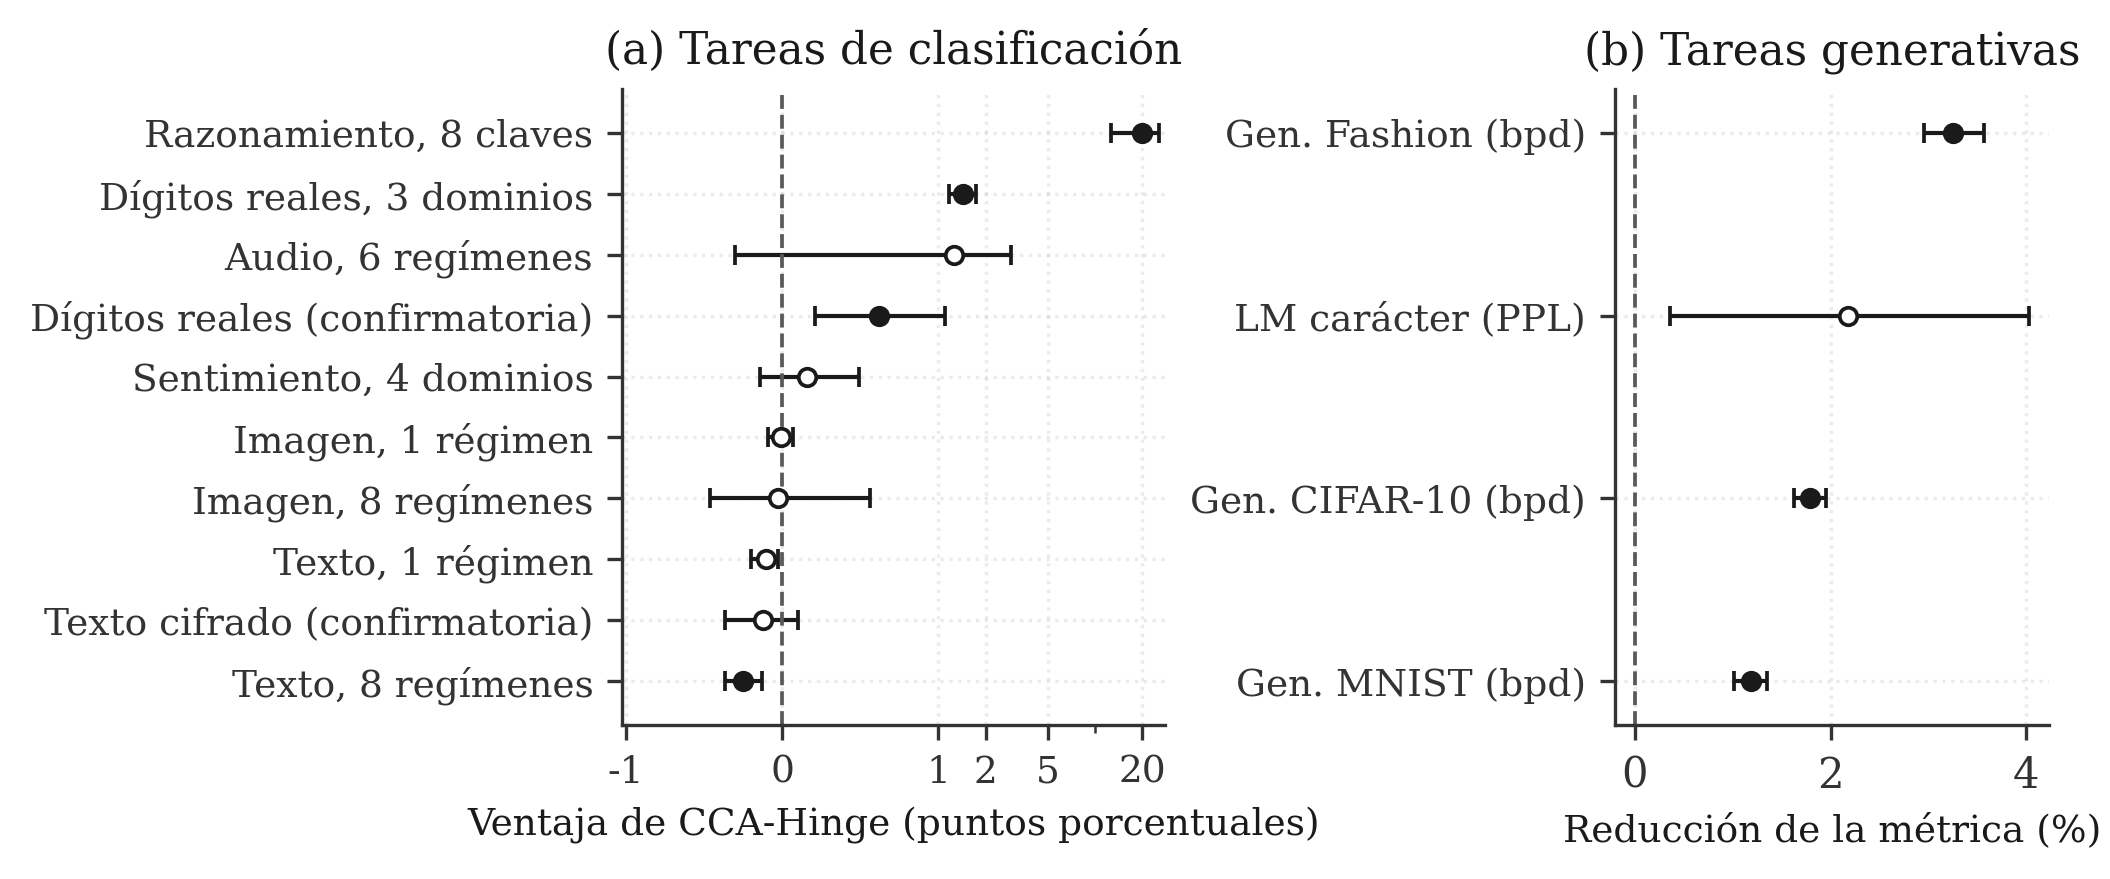
\includegraphics[width=0.84\textwidth]{figs/fig_bosque.png}
\caption{Ventaja de CCA-Hinge sobre Dynamic ReLU-B en cada tarea, con intervalos de confianza del $95\%$ sobre diez semillas emparejadas. Las entradas rotuladas \textit{confirmatoria} provienen de la Tabla~\ref{tab:matched} (semillas 3001--3010) y el resto de la Tabla~\ref{tab:matrix}. El marcador relleno indica diferencia significativa tras la corrección de Holm y el hueco, no significativa; el eje de (a) está comprimido de manera logarítmica más allá de $\pm1$. Las ganancias se concentran donde los regímenes exigen transformaciones distintas; en las tareas homogéneas el intervalo cruza el cero.}
\label{fig:bosque}
\end{figure*}

\subsection{¿De dónde proviene la ganancia?}

Que un método gane no explica por qué gana, y con una activación condicionada hay al menos dos explicaciones alternativas plausibles: que la ganancia venga de la información de contexto y no del mecanismo, o que el generador ni siquiera se aparte de su inicialización. Tres experimentos permiten descartarlas y atribuir la mejora al mecanismo propuesto.

El primero responde si alcanza con \textit{disponer} del contexto. El control de inyección directa recibe el mismo vector $c$ del mismo codificador, pero lo suma a la entrada en lugar de usarlo para deformar la curva, y rinde marcadamente peor: $13.88$ de perplejidad frente a $11.72$ en lenguaje por caracteres, $12.28\%$ frente a $49.88\%$ en razonamiento, y $0.955$, $1.350$ y $1.470$ bits por dimensión en generación frente a $0.937$, $1.284$ y $1.430$. Las cuatro diferencias son significativas sobre diez semillas ($p_{\mathrm{Holm}}=0.0117$). La información, por sí sola, no produce la ganancia: importa dónde se la aplica.

El segundo verifica que el modelo use el contexto \textit{correcto}. Al barajar los vectores de contexto entre muestras del mismo lote, CCA-Hinge cae de $88.05\%$ a $57.61\%$ en imágenes multirrégimen y de $88.96\%$ a $81.50\%$ en la mezcla real de dígitos, mientras que en el control de régimen único la misma perturbación casi no produce efecto ($98.49\%$ a $98.46\%$), que es lo que cabe esperar si no hay regímenes que distinguir. La activación depende, entonces, del resumen que corresponde a cada muestra; la prueba no demuestra que el modelo identifique el régimen en un sentido semántico, sino que su cómputo está efectivamente condicionado.

El tercero observa el interior del mecanismo. La Figura~\ref{fig:mecanismo} muestra, para un modelo CCA-Hinge entrenado en texto cifrado, las curvas generadas ante cinco regímenes, su diferencia respecto de la curva promedio y la varianza de cada coeficiente. Se observan tres hechos: la curva aprendida se aleja notablemente de SiLU, de modo que el generador no permanece en su inicialización; las curvas de distintos regímenes difieren entre sí, sobre todo donde la preactivación es grande en valor absoluto; y la adaptación se concentra en los coeficientes del numerador —$a_2$ es el más variable—, mientras los del denominador permanecen fijos. La red aprovecha así la libertad expresiva de la parametrización y conserva intacto el término que garantiza su estabilidad numérica.

\begin{figure*}[t]
\centering
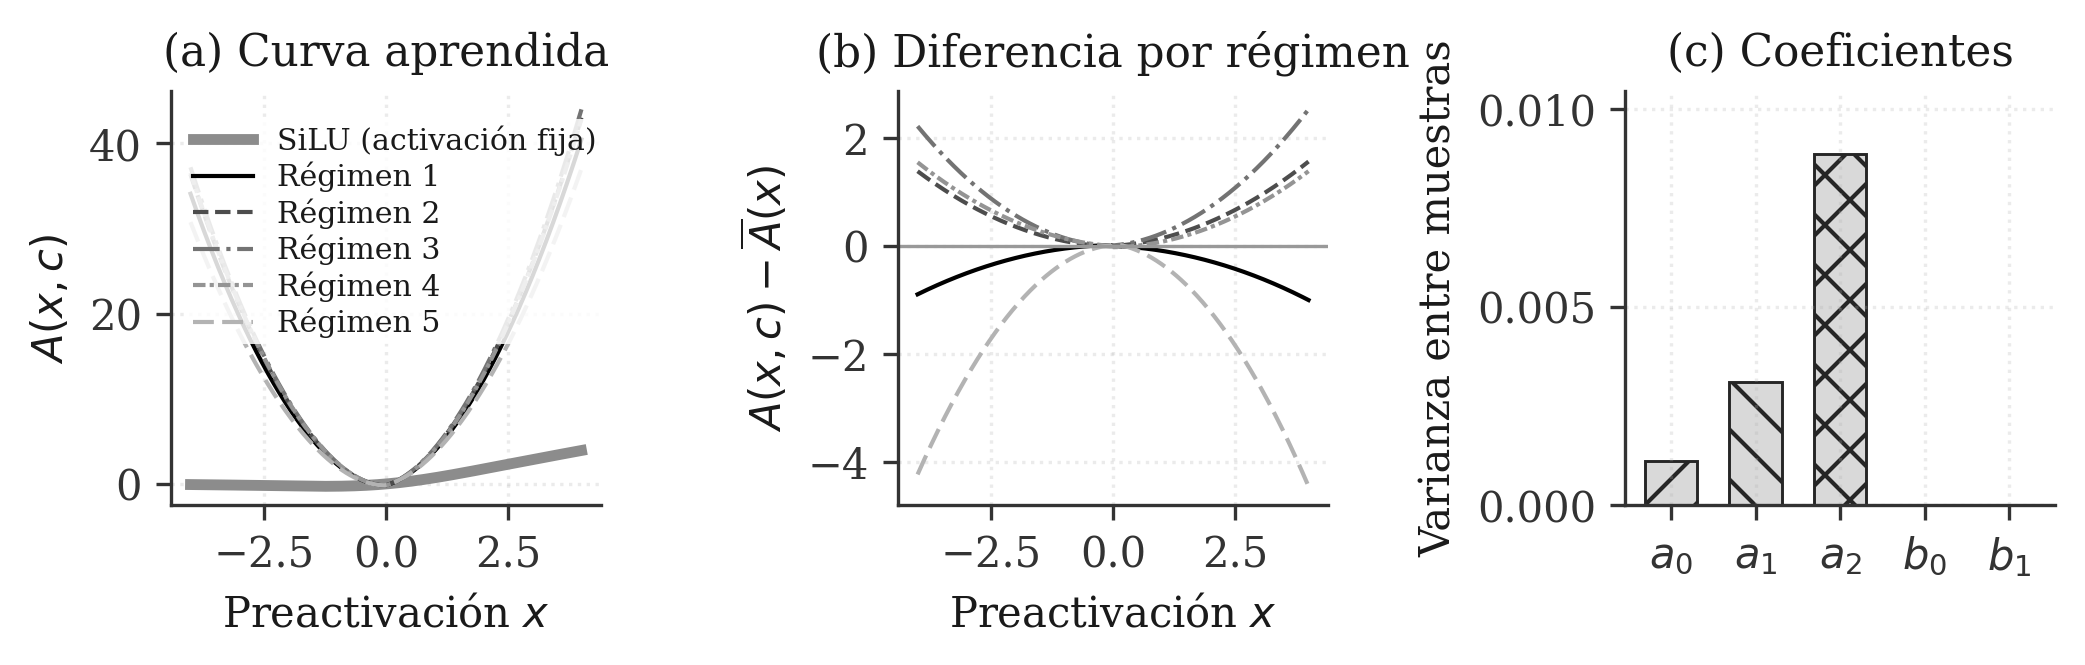
\includegraphics[width=0.86\textwidth]{figs/fig_mecanismo.png}
\caption{Mecanismo interno de CCA-Hinge en la tarea de texto cifrado. (a) Curva generada para cinco regímenes frente a la SiLU fija. (b) Diferencia de cada curva respecto del promedio, que hace visible la adaptación. (c) Varianza de cada coeficiente entre muestras: la red modifica el numerador y deja fijo el denominador.}
\label{fig:mecanismo}
\end{figure*}

\subsection{¿Cuánto cuesta?}

Una activación más compleja sólo resulta útil si su costo es tolerable, y conviene ser explícito al respecto porque es la objeción más inmediata a la propuesta. Las tres últimas columnas de la Tabla~\ref{tab:matched} miden el tiempo de una iteración de propagación y gradiente con lotes de 256 muestras, sobre esas mismas configuraciones de presupuesto igualado, en una GPU NVIDIA L4, en modo interpretado (\textit{eager}) y compilado con \texttt{torch.compile} \cite{ansel2024pytorch2}.

\textbf{El sobrecosto es de lanzamiento, no aritmético.} En modo interpretado, CCA-Hinge cuesta $4.75$ veces lo que la SiLU igualada en texto y $5.78$ veces en dígitos. Esa penalización no proviene del trabajo aritmético: sus operaciones por muestra son apenas un $6.3\%$ mayores en texto y un $1.6\%$ \textit{menores} en dígitos, donde la búsqueda de presupuesto compensa el generador con una red anfitriona más angosta. La distancia entre ambos factores —casi seis veces más lento con la misma cantidad de cuentas— mide el costo de ejecutar decenas de operaciones puntuales diminutas como núcleos de GPU separados.

\textbf{La compilación recupera la mayor parte.} Al fusionar esas operaciones, CCA-Hinge obtiene la mayor aceleración de la tabla ($2.25\times$ y $2.97\times$), por ser el método con más trabajo puntual fusionable; el efecto crece con la complejidad de la activación, y la SiLU igualada, que no tiene nada que fusionar, incluso se degrada ($0.88\times$ y $0.92\times$). El sobrecosto compilado frente a ella baja así a $1.85\times$ y $1.79\times$, y frente a Dynamic ReLU-B queda en $+13.4\%$ y $+6.5\%$: sobre la mezcla real de dígitos, ese $6.5\%$ adicional compra $0.62$ puntos de exactitud frente al mejor competidor y $7.5$ frente a la SiLU igualada.

\textbf{Alcance de la medición.} La compilación reduce el costo en estado estacionario, no el de estas corridas: su calentamiento de 20 a 27 segundos no se amortiza en entrenamientos cortos. La exactitud no depende del hardware y se conserva de la corrida original; el costo sí, y por eso se remidió en una sola máquina. No afirmamos que estas proporciones se mantengan en otras GPU ni en modelos mayores.

\section{Trabajos Relacionados}

La idea de que la no linealidad no tiene por qué ser fija no es nueva, y ha seguido dos caminos que hasta ahora corrieron bastante separados y que este trabajo articula.

El primero busca \textit{aprender} la curva, y la escala del problema es considerable: un relevamiento reciente cataloga más de cuatrocientas funciones de activación propuestas en tres décadas \cite{kunc2024threedecades}, lo que da una medida tanto del interés sostenido en el tema como de la dificultad de establecer cuáles aportan una mejora real. PReLU \cite{he2015prelu} aprende la pendiente de la rama negativa y muestra que un grado mínimo de libertad ya mejora el resultado; Maxout \cite{goodfellow2013maxout} generaliza la idea tomando el máximo de varias ramas lineales, a costa de multiplicar los parámetros; y la búsqueda automática de activaciones \cite{ramachandran2017swish} derivó en Swish y en la adopción de curvas suaves como SiLU \cite{silu} o GELU \cite{hendrycks2016gelu}. Las unidades racionales aportan un argumento teórico —aproximan funciones suaves con menor profundidad que una red ReLU equivalente \cite{boulle2020rational}— las de Padé muestran que pueden entrenarse de extremo a extremo \cite{molina2020pade} y su uso en aprendizaje por refuerzo sugiere que la plasticidad de la curva importa sobre todo cuando la distribución de entrada cambia \cite{delfosse2024adaptive}, mientras que las redes de Kolmogórov--Arnold \cite{liu2024kan} aprenden una función univariada en cada arista, aunque evaluaciones posteriores que controlan parámetros y costo encuentran que su ventaja se limita a la regresión simbólica y no se sostiene en visión ni en lenguaje \cite{hou2024kanassessment}, un antecedente que ilustra por qué aquí insistimos en el presupuesto igualado. Todas comparten una limitación: la curva es única para todo el conjunto y queda congelada en inferencia, de modo que un modelo entrenado sobre regímenes heterogéneos debe resolverlos con un único compromiso.

El segundo camino es el cómputo condicionado, donde una parte de la red produce o selecciona parámetros de otra en función de la entrada \cite{bengio2013conditional}; el área está sistematizada en el relevamiento de redes neuronales dinámicas \cite{han2022dynamic}, que distingue el condicionamiento por muestra, por región espacial y por profundidad, y dentro del cual CCA pertenece al primero. Las hiperredes \cite{ha2017hypernetworks} generan los pesos de la red principal; FiLM \cite{perez2018film} modula las características intermedias mediante escalas y desplazamientos condicionados; CondConv \cite{yang2019condconv} combina núcleos convolucionales con pesos que dependen de la muestra; y las mezclas de expertos dispersas \cite{shazeer2017moe} encaminan cada ejemplo hacia un subconjunto de especialistas, un esquema hoy vigente en modelos de lenguaje de gran escala \cite{jiang2024mixtral}. Todas condicionan los pesos o las representaciones, pero dejan intacta la forma de la no linealidad, que es el componente sobre el que actúa CCA. La distinción no es sólo conceptual: el control de inyección directa recibe la misma información de contexto y la incorpora a la representación —como haría una modulación al estilo FiLM—, y aun así rinde significativamente peor, lo que muestra que el punto de aplicación importa.

En la intersección de ambos caminos se ubican los comparadores directos de este trabajo. Dynamic ReLU \cite{chen2020dynamic} genera desde un resumen global los coeficientes de dos ramas lineales y devuelve su máximo, con lo que obtiene una envolvente lineal por tramos adaptada a la entrada; ACON y su versión Meta-ACON \cite{ma2021activate} reinterpretan la activación como una transición suave entre dos ramas y condicionan el factor que la regula. CCA se diferencia en que condiciona a la vez un reencuadre afín y una corrección racional acotada, y en que CCA-Hinge incorpora una base de quiebre suave que recupera la capacidad de Maxout sin renunciar a la inicialización exacta en SiLU. Nuestra comparación implementa las tres formulaciones sobre una interfaz común y les entrega idéntico contexto, condición que rara vez se cumple en los reportes originales.

Queda un aspecto metodológico que ninguna de estas líneas resuelve: las ventajas de las activaciones adaptativas suelen informarse sin igualar el presupuesto y sin análisis estadístico pareado, prácticas cuya influencia sobre las conclusiones está documentada \cite{bouthillier2021accounting}. Parte de la contribución de este artículo es mostrar qué queda de esas ventajas bajo presupuesto igualado, semillas emparejadas, corrección por comparaciones múltiples \cite{holm1979simple} y controles negativos explícitos; el hallazgo de que la técnica no mejora a una activación fija en el problema real de sentimiento es tan parte del resultado como las ganancias multirrégimen. CCA tampoco compite con las técnicas de adaptación de dominio o de transferencia, que requieren conocer o etiquetar los dominios: aquí el régimen se infiere de la propia actividad de la red.

\section{Conclusión y Trabajos Futuros}

Este trabajo se propuso determinar si conviene adaptar la no linealidad de una red al contexto de cada muestra, y a qué costo. La respuesta es afirmativa, pero acotada, y esa delimitación —más que la ganancia en sí— es su principal aporte. Bajo presupuesto igualado y sobre semillas no utilizadas en el diseño, CCA-Hinge supera significativamente a Dynamic ReLU-B en el banco real formado por MNIST, SVHN y USPS y en las tres tareas de generación de imágenes, y obtiene la mejor media en razonamiento modular. En audio, con presupuesto igualado, queda por detrás de la racional estática. En texto queda empatada con los métodos adaptativos en la tarea confirmatoria y un cuarto de punto por debajo de Dynamic ReLU-B en la matriz con presupuesto igualado, y en el análisis de sentimiento multi-dominio no mejora a una SiLU fija. La regla que emerge es utilizable en la práctica: condicionar la forma de la activación conviene cuando el contexto modifica la transformación necesaria, y agregar complejidad dinámica a un problema homogéneo no garantiza beneficio alguno. Los tres controles sostienen además que la mejora proviene del mecanismo de condicionamiento y no del mero acceso a la información.

El estudio tiene limitaciones que conviene explicitar. Las redes anfitrionas son pequeñas, de decenas de miles de parámetros, y no evaluamos modelos fundacionales, por lo que las proporciones de costo y de ganancia no pueden extrapolarse sin más. La generación de imágenes se limita a 500 pasos, un régimen corto que privilegia la rapidez del experimento. La equivalencia estricta de recursos se verifica en las dos tareas de la Tabla~\ref{tab:matched} y en las cinco de clasificación marcadas en la Tabla~\ref{tab:matrix}; las restantes conservan la red anfitriona original, con diferencias de parámetros que el código publicado detalla. Tampoco evaluamos cambios de dominio no observados durante el entrenamiento, un escenario frecuente en producción.

Cada limitación sugiere una continuación: replicar la comparación con presupuesto igualado sobre transformadores de tamaño medio, donde el costo relativo del generador es menor; medir el comportamiento ante regímenes nunca vistos, que es donde la inferencia del contexto podría fallar; escribir un núcleo fusionado a medida, ya que la penalización es de lanzamiento y no aritmética; y caracterizar qué codifica el vector de contexto, pues el barajado demuestra dependencia del contexto correcto pero no identificación semántica del régimen.

\ifanonima
El código, las configuraciones, los resultados por semilla, los manifiestos SHA-256 y los comandos de reproducción estarán disponibles en el repositorio público del proyecto tras el proceso de evaluación anónima. Las corridas de exactitud usaron PyTorch 2.11 sobre una NVIDIA RTX 4070 Laptop; las diez semillas de generación y las mediciones de costo, PyTorch 2.8 sobre una NVIDIA L4, y cada bloque de diez semillas proviene de una única máquina. Los datos no se redistribuyen: se descargan de sus fuentes originales conservando las particiones descritas.
\else
El código, las configuraciones, los resultados por semilla, los manifiestos SHA-256 y los comandos de reproducción están disponibles en el repositorio público del proyecto.\footnote{\url{https://github.com/agustinastie2/Context-Conditioned-Rational-Activations}} Las corridas de exactitud usaron PyTorch 2.11 sobre una NVIDIA RTX 4070 Laptop; las diez semillas de generación y las mediciones de costo, PyTorch 2.8 sobre una NVIDIA L4, y cada bloque de diez semillas proviene de una única máquina. Los datos no se redistribuyen: se descargan de sus fuentes originales conservando las particiones descritas.
\fi

\renewcommand\refname{Referencias}
\bibliographystyle{ieeetr}
\bibliography{referencias}

\ifanonima\else
\miniseccion{Datos de Contacto}

{\footnotesize\raggedright
\textit{Agustín H. Astie Forconesi. Universidad del Aconcagua, Catamarca 147, M5500 Mendoza, Argentina. \texttt{agustinastie3@gmail.com}}\par}
\fi

\end{multicols}

\end{document}
